\pagebreak
\section{Data Types}

  \subsection{Base Data Types}
  \label{sect:ivoa}
  Provides a set of standardized primitive data types as well as types for representing quantities
( values with associated units ). We provide a diagram of the model here, and refer the reader to
Section 5 of the VO-DML modeling specification document \citep{std:VODML} for more information.


    \begin{figure}[h]
    \begin{center}
      \fbox{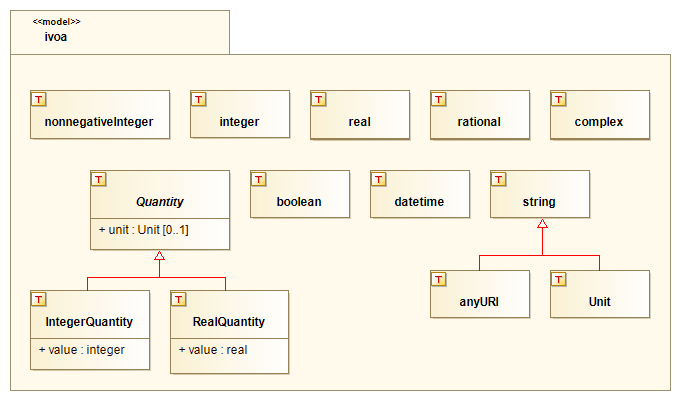
\includegraphics[width=\textwidth-0.1in]{diagrams/ivoa_types.png}}
      \caption{Base Data Types}\label{fig:basetypes}
    \end{center}
    \end{figure}


  \subsubsection{Units}
  \label{sect:Units}
  This model requires the use of the IVOA VOUnits Standard \citep{std:VOUNIT} for representing units of physical
quantities. This standard reconciles common practices and current standards for use within the
IVOA community.

  \subsubsection{Dates}
  \label{sect:Dates}
  The 'datetime' datatype is for expressing date-time values. The string representation of a
datetime value should follow the FITS convention for representing dates. The FITS standard is
effectively ISO8601 format without the "Z" tag to indicate UTC (YYYY-MM-DDThh:mm:ss).
Values are nominally expressed in UTC.
